\documentclass[11pt,a4paper]{article}
\usepackage[margin=27mm,top=26mm,bottom=24mm,headheight=14pt,headsep=7mm]{geometry}
\usepackage{amsmath,amsthm,booktabs,graphicx,luatexja-fontspec,unicode-math}
\setmainfont{LibertinusSerif-Regular.otf}[
  BoldFont=LibertinusSerif-Bold.otf,ItalicFont=LibertinusSerif-Italic.otf,
  BoldItalicFont=LibertinusSerif-BoldItalic.otf]
\setmathfont{LibertinusMath-Regular.otf}
\setmonofont{lmmono10-regular.otf}[Scale=MatchLowercase]
\setmainjfont{HaranoAjiMincho-Regular.otf}[BoldFont=HaranoAjiMincho-Bold.otf]
\usepackage{xcolor,fancyhdr}
\usepackage[labelsep=period]{caption}
\definecolor{link}{HTML}{185B65}
\usepackage[unicode,colorlinks=true,linkcolor=link,citecolor=link,urlcolor=link]{hyperref}
\hypersetup{pdftitle={The mass-volume-area hierarchy for Kerr black holes in f(R) gravity},
  pdfauthor={Naoki Takata},pdfsubject={Thermodynamic volume, Kerr black holes and Lean formalization},
  pdfdisplaydoctitle=true}
\pagestyle{fancy}\fancyhf{}
\fancyhead[L]{\small\itshape The mass--volume--area hierarchy for Kerr black holes}
\fancyhead[R]{\small Naoki Takata}
\fancyfoot[C]{\small\thepage}
\renewcommand{\headrulewidth}{0.3pt}
\fancypagestyle{firstpage}{\fancyhf{}\fancyfoot[C]{\small\thepage}\renewcommand{\headrulewidth}{0pt}}
\setlength{\parindent}{1.15em}
\setlength{\parskip}{1.5pt}
\setlength{\abovedisplayskip}{7pt plus 2pt minus 1pt}
\setlength{\belowdisplayskip}{7pt plus 2pt minus 1pt}
\setlength{\jot}{4pt}
\raggedbottom
\newcommand{\VE}{V_{\mathrm E}}
\newcommand{\PE}{P_{\mathrm E}}
\newcommand{\HE}{H_{\mathrm E}}
\newcommand{\repo}{https://github.com/nktkt/blackhole}
\newcommand{\proofref}[3]{\href{\repo/blob/kerr-volume-hierarchy-v1/BlackHole/#1.lean\#L#3}{\texttt{\detokenize{#2}}}}

\begin{document}
\thispagestyle{firstpage}
\begin{center}
  {\LARGE\bfseries The mass--volume--area hierarchy for\\[2pt]
  Kerr black holes in \(f(R)\) gravity\par}
  \vspace{10pt}
  {\large Naoki Takata\par}
  \vspace{3pt}
  {25 November 2026\par}
\end{center}

\begin{abstract}
Thermodynamic volume at zero cosmological constant depends on how the mass varies along a family of solutions. We compute this response on the vacuum Einstein branch of \(f(R)-2\Lambda\) gravity at fixed Wald entropy and angular momenta. For \(f(0)=0\) and \(f'(0)=1\), the flat volume differs from its Einstein value by \(-16\pi D M f''(0)/(D-2)^2\). In four dimensions we obtain a closed interval for \(f''(0)\) from the horizon area and angular momentum of each uncharged Kerr black hole. Its lower and upper endpoints correspond to saturation of the mass and area bounds, respectively. The full subextremal family, including Schwarzschild, obeys both bounds exactly when \(f''(0)=0\). The pressure derivative and the coupling classification have been formalized in Lean~4.
\end{abstract}

\section{The flat-space question}\label{sec:question}
Mann, Pourhassan and Dehghani ask under which conditions the Penrose and reverse isoperimetric ratios of an asymptotically flat black hole obey their Eq.~(51)~\cite{mann}. In units \(G=1\), let \(\omega\) be the area of the unit \((D-2)\)-sphere. For mass \(M>0\), geometric horizon area \(A>0\), and thermodynamic volume \(V\geq0\), define
\begin{equation}\label{eq:radii}
 r_A=\left(\frac{A}{\omega}\right)^{\!1/(D-2)},\quad
 r_V=\left(\frac{(D-1)V}{\omega}\right)^{\!1/(D-1)},\quad
 r_M=\left(\frac{16\pi M}{(D-2)\omega}\right)^{\!1/(D-3)} .
\end{equation}
The two ratios are \(r_M/r_A\) and \(r_V/r_A\), respectively. For \(D\geq4\), their hierarchy reads \(r_A\leq r_V\leq r_M\). Since the volume of a ball increases with its radius, this is equivalent to
\begin{equation}\label{eq:bounds}
 V_A\leq V\leq V_M,\qquad V_A=\frac{\omega r_A^{D-1}}{D-1},\qquad
 V_M=\frac{\omega r_M^{D-1}}{D-1}.
\end{equation}
The extended first law identifies \(V\) with the pressure derivative of the enthalpy at fixed entropy and conserved charges~\cite{cvetic,dolan}. We vary the bare cosmological constant through \(P=-\Lambda/(8\pi)\), keep every coupling in \(f\) fixed, and take the right derivative at \(P=0\) from the anti-de Sitter side. A flat Kerr metric fixes \(A\) and \(M\). The derivative in this experiment also probes the gravitational action. The classification below is for the uncharged Einstein branch of the specified \(f(R)\) theories. The general classification posed in Ref.~\cite{mann} remains open.

\smallskip
{\small\noindent\textbf{日本語要旨}\quad
真空アインシュタイン解として圧力を変化させると、平坦極限の熱力学的体積には \(f''(0)\) に比例する補正が生じる。各Kerr解で質量・体積・面積の不等式が成立する結合定数の範囲を求めた。回転ゼロを含む全非極限Kerr解で成立するための必要十分条件は \(f''(0)=0\) である。\par}

\newpage
\section{Volume at fixed physical charges}\label{sec:shift}
Consider the vacuum action \((16\pi)^{-1}\int \sqrt{-g}\,[f(R)-2\Lambda]\,d^D x\). Assume \(f\) is \(C^2\) near zero, \(f(0)=0\), and \(f'(0)=1\). Take a family of Einstein metrics with \(R_{\mu\nu}=(R/D)g_{\mu\nu}\) and constant scalar curvature on each spacetime. Write \(x=(S,J_1,\ldots,J_k)\) for the physical extensive variables. Assume the reference Einstein enthalpy \(\HE(p,x)\) has a differentiable local extension at \(p=0\) and satisfies the uncharged vacuum Smarr relation there. These hypotheses allow rotation and any number of angular momenta.

\paragraph{Curvature response.}
The trace equation reduces to \(Rf'(R)-\tfrac D2[f(R)+16\pi P]=0\). The bare pressure and the pressure of the same metric in Einstein gravity are therefore
\begin{equation}\label{eq:trace}
 P(R)=\frac{2Rf'(R)/D-f(R)}{16\pi},\qquad
 \PE(R)=-\frac{D-2}{16\pi D}\,R .
\end{equation}
These functions have the same nonzero slope at zero. The inverse function theorem gives a local curvature branch \(R(P)\) through zero. With \(q=f''(0)\) and \(F(P)=f'(R(P))\), its derivatives are
\begin{equation}\label{eq:slopes}
 R'(0)=-\frac{16\pi D}{D-2},\qquad
 (\PE\circ R)'(0)=1,\qquad F'(0)=-\frac{16\pi D}{D-2}\,q .
\end{equation}
Here \(F(0)=1\), so \(F>0\) in a neighborhood of the endpoint.

\paragraph{Theorem 1.}
\emph{For the fixed-charge pressure variation described above, the flat thermodynamic volume satisfies}
\begin{equation}\label{eq:shift}
 \boxed{\displaystyle V_f=\VE-C_D(M)q,\qquad
 C_D(M)=\frac{16\pi D\,M}{(D-2)^2}.}
\end{equation}
Here \(M=\HE(0,x)\) and \(\VE=\partial_p\HE(0,x)\).

\paragraph{Proof.}
For the same metric and normalization of the asymptotic Killing fields, the conserved mass and angular momenta carry the common factor \(F\). The Wald entropy carries the same factor on a constant-\(R\) horizon~\cite{koga}. The physical enthalpy at fixed \(x\) is consequently
\begin{equation}\label{eq:enthalpy}
 H_f(P,x)=F(P)\,\HE\bigl(\PE(R(P)),x/F(P)\bigr).
\end{equation}
Differentiation at zero gives \(V_f=\VE+F'(0)[M-D_x\HE(0,x)[x]]\). At zero pressure the Smarr relation reads \((D-2)D_x\HE(0,x)[x]=(D-3)M\), since the directional derivative is \(TS+\sum_i\Omega_iJ_i\). The bracket is \(M/(D-2)\), which gives Eq.~\eqref{eq:shift}. \hfill\qedsymbol

For a positive-mass seed, \(C_D(M)>0\). Combining Eqs.~\eqref{eq:bounds} and \eqref{eq:shift} gives the closed interval
\begin{equation}\label{eq:general}
 \frac{\VE-V_M}{C_D(M)}\ \leq\ q\ \leq\ \frac{\VE-V_A}{C_D(M)} .
\end{equation}
The lower endpoint gives \(V_f=V_M\), and the upper endpoint gives \(V_f=V_A\). The area bound already enforces the nonnegative-volume domain of Eq.~\eqref{eq:radii}.

The coefficient also has a converse interpretation. For a given positive-mass seed and any prescribed positive \(V_*\), the polynomial \(f(R)=R+\alpha R^2+\beta R^3\) realizes \(V_f=V_*\) when \(\alpha=(\VE-V_*)/(2C_D(M))\). Each such action uses the same flat charges and may have the same \(\beta\).

\newpage
\section{The Kerr classification}\label{sec:kerr}
For uncharged Kerr in \(D=4\), set \(s=S/\pi\), \(j=2J\), and \(b=8\pi/3\). In these coordinates the Einstein enthalpy of Kerr--AdS, Eq.~(19) of Dolan~\cite{dolan}, is
\begin{equation}\label{eq:dolan}
 \HE(p,s,j)=\tfrac12\sqrt{s(1+bps)^2+\frac{j^2}{s}(1+bps)} .
\end{equation}
At the flat endpoint \(S=A/4\). Define the area radius \(\rho\), signed spin \(\chi\), and positive factor \(t\) by
\begin{equation}\label{eq:spin}
 \rho=\sqrt{s}=\sqrt{A/(4\pi)},\qquad
 \chi=j/s=8\pi J/A,\qquad t=\sqrt{1+\chi^2}.
\end{equation}
The flat Kerr relations \(2Mr_+=r_+^2+a^2=A/(4\pi)\) and \(J=Ma\) give \(\chi=a/r_+\). Conversely, \(r_+=\rho/t\) and \(a=\chi\rho/t\). Thus \(\rho>0\) and \(|\chi|<1\) parameterize the subextremal outer horizons, including Schwarzschild at \(\chi=0\).

\paragraph{Theorem 2.}
\emph{For a subextremal Kerr seed on this branch, both bounds in Eq.~\eqref{eq:bounds} hold precisely when}
\begin{equation}\label{eq:kerr}
 \boxed{\displaystyle
 -\frac{\rho^2(t^2-1)(2t^2+1)}{12t^2}
 \ \leq\ f''(0)\ \leq\
 \frac{\rho^2(t-1)^2}{12t^2}.}
\end{equation}
\paragraph{Proof.}
Evaluating Eq.~\eqref{eq:dolan} at zero pressure gives \(M=\rho t/2\). At \(p=0\), multiplying \((s,j)\) by a common positive factor \(u\) multiplies \(\HE\) by \(\sqrt{u}\). Differentiating with respect to \(u\) at \(u=1\) verifies \(2D_x\HE(0,x)[x]=M\) directly. Differentiating the same enthalpy with respect to \(p\) instead, at fixed \(s,j\), yields
\begin{equation}\label{eq:VE}
 \VE=\frac{\pi(2s^2+j^2)}{3M}
     =\frac{2\pi\rho^3(1+t^2)}{3t}.
\end{equation}
The geometric endpoints and the response coefficient are
\begin{equation}\label{eq:kerrvol}
 V_A=\frac{4\pi\rho^3}{3},\qquad
 V_M=\frac{4\pi(\rho t)^3}{3},\qquad
 C_4(M)=16\pi M=8\pi\rho t .
\end{equation}
Substitution into Eq.~\eqref{eq:general} yields Eq.~\eqref{eq:kerr}. \hfill\qedsymbol

\paragraph{Corollary.}
\emph{For a fixed action, the hierarchy holds throughout the four-dimensional subextremal Kerr family if and only if \(f''(0)=0\).}
Indeed, \(t=1\) for a nonrotating member and the interval then reduces to \(\{0\}\). Conversely, \(t\geq1\) at every spin, so zero belongs to every interval. In particular, for \(f(R)=R+\alpha R^2+\beta R^3\) the family-wide condition is \(\alpha=0\), with \(\beta\) arbitrary. This result concerns the first pressure derivative at the flat endpoint. At finite pressure the factor \(f'(R(P))\) also samples higher powers of curvature.

\newpage
\section{How rotation separates the two bounds}
At fixed \(\rho\), increasing \(q=f''(0)\) decreases the volume by Eq.~\eqref{eq:shift}. A sufficiently negative coupling therefore takes the solution through the mass bound. A sufficiently positive coupling takes it through the area bound. The thresholds scale differently near the nonrotating limit. Writing \(\gamma=q/\rho^2\), expansion of Eq.~\eqref{eq:kerr} gives
\begin{equation}\label{eq:slow}
 \gamma_{\min}=-\frac{\chi^2}{4}+O(\chi^4),\qquad
 \gamma_{\max}=\frac{\chi^4}{48}+O(\chi^6).
\end{equation}
The positive side of the allowed interval opens only at fourth order in spin. Figure~\ref{fig:interval} displays both thresholds, with a separate scale for the upper one.

\begin{figure}[ht]
 \centering
 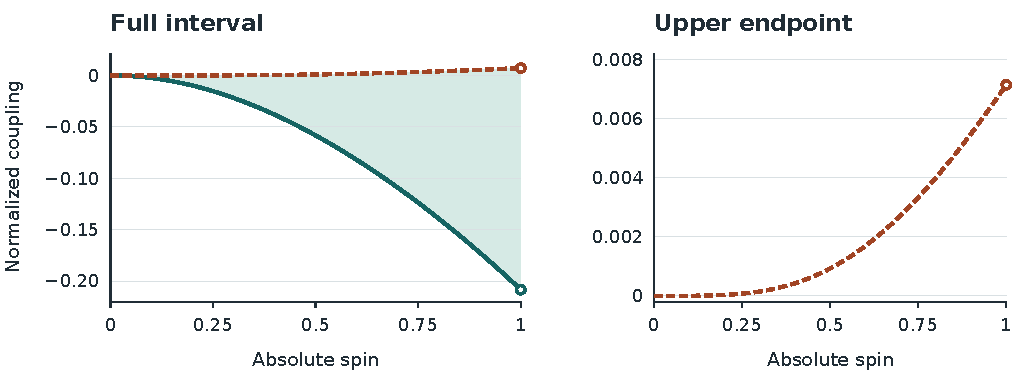
\includegraphics[width=0.98\linewidth]{figures/coupling-interval.pdf}
 \caption{Normalized coupling \(f''(0)/\rho^2\) against \(|\chi|=|a|/r_+\). The shaded band is the allowed interval. The solid curve marks \(V_f=V_M\) and the dashed curve marks \(V_f=V_A\). The right panel expands the vertical scale of the upper endpoint. Open circles mark the limit \(|\chi|\to1\) of the subextremal family.}
 \label{fig:interval}
\end{figure}

\paragraph{An exact rotating example.}
Take \(\rho=4\) and \(|\chi|=3/4\), giving \(t=5/4\) and \(M=5/2\). The Einstein volume is \(1312\pi/15\), while \(V_A=256\pi/3\) and \(V_M=500\pi/3\). Since \(V_f=1312\pi/15-40\pi q\), the hierarchy is equivalent to
\[
 -\frac{99}{50}\leq q\leq\frac{4}{75}.
\]
These rational endpoints also follow by direct substitution into Eq.~\eqref{eq:kerr}.

\paragraph{A nonrotating check.}
For \(f(R)=R+\alpha R^2\), a Schwarzschild horizon of areal radius \(r\) has \(M=r/2\) and identical endpoint volumes \(4\pi r^3/3\). Equation~\eqref{eq:shift} gives \(V_f=4\pi r^3/3-16\pi\alpha r\). At \(r=4,\ \alpha=1\), the physical volume is \(64\pi/3\), strictly positive and below the area bound \(256\pi/3\). Thus two actions that coincide in their flat mass and area can assign different values to the flat pressure response.

\newpage
\section{Formal verification and scope}
The Lean development uses the right derivative on \(P\geq0\). It constructs the local scalar-curvature branch by the inverse function theorem, differentiates the fixed-charge enthalpy, and checks both inequalities including their equality cases. The physical inputs are the Einstein-branch charge and entropy normalization, the existence of a differentiable Einstein enthalpy chart, and the reference Smarr relation. For Kerr, the chart is Eq.~\eqref{eq:dolan} and the proof derives its Smarr identity. Field-equation existence for general stationary metrics and dynamical stability lie outside these hypotheses.

\begin{center}
\small
\begin{tabular}{@{}ll@{}}
\toprule
Mathematical statement & Lean declaration \\
\midrule
Pressure response, Eq.~\eqref{eq:shift} & \proofref{ScalarCurvatureGravity}{volume_shift}{144}\\
General interval, Eq.~\eqref{eq:general} & \proofref{ScalarCurvatureGravity}{hierarchy_iff_second}{197}\\
Kerr interval, Eq.~\eqref{eq:kerr} & \proofref{KerrScalarCurvature}{kerr_iff}{97}\\
All subextremal Kerr states & \proofref{KerrScalarCurvature}{all_kerr_iff}{159}\\
Polynomial actions & \proofref{KerrScalarCurvature}{all_kerr_polynomial_iff}{179}\\
\bottomrule
\end{tabular}
\end{center}

\paragraph{Beyond the Kerr chart.}
Let \(m(P,u)\) be the mass of a state \(u\), with the field equations, boundary data and fixed charges represented by \(G(P,u)=0\). At the flat solution put \(L=D_uG\), \(b=\partial_PG\), and \(\ell=D_um\). The tangent \(v\) to a differentiable solution branch satisfies \(Lv=-b\). If a linear functional \(\eta\) satisfies \(\ell=\eta\circ L\), then \(V=\partial_Pm-\eta(b)\). On a nonempty linearized fiber such a multiplier exists exactly when \(\ker L\subseteq\ker\ell\). In infinite dimensions the multiplier here is algebraic.

The quadratic example also distinguishes exact tests from finite approximations. Fix \(r=4\). For a program on input zero, set \(\alpha=2^{-(k+1)}\) if its first successful bounded simulation has cutoff \(k\), and \(\alpha=0\) if it never halts. Scanning the first \(N\) cutoffs gives a rational approximation with error at most \(2^{-N}\). All these volumes are positive, and the hierarchy is equivalent to \(\alpha=0\). An exact decision procedure for every such program would therefore decide nonhalting. A rational supplied as a numerator and denominator admits a direct zero test. The \href{\repo/tree/kerr-volume-hierarchy-v1}{versioned proof repository} includes the reduction and build instructions for Lean and mathlib 4.29.1.

\paragraph{Acknowledgment.}
OpenAI Codex assisted with the manuscript, the Lean formalization and the verification workflow.

\begin{thebibliography}{9}\small
\bibitem{mann} R.~B. Mann, B.~Pourhassan and A.~Dehghani,
\emph{On the Classical, Penrose, and Reverse Isoperimetric Inequalities in Black Holes: Insights From AdS to Flat Riemannian Backgrounds} (2026).
\href{https://arxiv.org/html/2609.14108v1#S5.E51}{arXiv:2609.14108v1, Eq.~(51)}.
\bibitem{cvetic} M.~Cvetič, G.~W. Gibbons, D.~Kubizňák and C.~N. Pope,
\emph{Black Hole Enthalpy and an Entropy Inequality for the Thermodynamic Volume}.
\href{https://doi.org/10.1103/PhysRevD.84.024037}{Phys. Rev. D \textbf{84}, 024037 (2011)}.
\bibitem{dolan} B.~P. Dolan, \emph{Pressure and volume in the first law of black hole thermodynamics}.
\href{https://doi.org/10.1088/0264-9381/28/23/235017}{Class. Quantum Grav. \textbf{28}, 235017 (2011)}.
\href{https://arxiv.org/html/1106.6260#S2.E19}{Eq.~(19)}.
\bibitem{koga} J.~Koga, \emph{The first law of AdS black holes in higher curvature gravity}.
\href{https://doi.org/10.1103/PhysRevD.72.064010}{Phys. Rev. D \textbf{72}, 064010 (2005)}.
\href{https://arxiv.org/html/hep-th/0505219#S2.E6}{Eq.~(6)} and
\href{https://arxiv.org/html/hep-th/0505219#S3.E48}{Eqs.~(47)--(48)}.
\end{thebibliography}
\end{document}
